\section{Lustre Architecture}

\subsection{Network Architecture}

The Lustre architechtecture aims to connect a number of clients with the data
servers in an efficient and failsafe way. The following graph shows an example
structure of the network setup in a Lustre environment.

\iffinal
    \begin{figure}[htb]
        \centering
        \tikzset{
            area/.style=    { draw=black!30!white, dashed, very thick, rounded corners=3pt },
            highlight/.style = { fill=yellow!50!white, rounded corners=3pt },
            node/.style =   { circle, inner sep=0pt, minimum size=15pt },
            client/.style = { node, fill=RoyalBlue },
            mds/.style =    { node, fill=YellowGreen },
            mdt/.style =    { node, fill=Dandelion },
            oss/.style =    { node, fill=OliveGreen },
            ost/.style =    { node, fill=BrickRed },
            link/.style =   { line width=1.5pt, line cap=rect },
            olink/.style =  { link, draw=Red },
            mlink/.style =  { link, draw=Dandelion!50!white },
            net/.style =    { link, line width=2pt },
            net1/.style =   { net, draw=black!20!white },
            net2/.style =   { net, draw=black!50!white },
            failover/.style={
                %decoration={markings,mark=at position 1 with {\arrow{triangle 60}},scale=0.5},
                %postaction=decorate,
                line width=1.0pt,
                -stealth,
            },
            failover'/.style={
                failover,
                stealth-stealth
            },
        }

        \makebox[\textwidth][c] {
            \begin{tikzpicture}[y=-1.2cm,x=1.2cm]

                \draw[area]
                    (-5.5, -0.5) rectangle (2.5, 0.5)
                    (-5.5, 1) rectangle (-3.4, 4.0)
                    (-5.5, 4.5) rectangle (4.5, 6.5)
                    ;

                \node[anchor=west] (clients)  at (-5.5, 0.0) {\scriptsize CLIENTS};
                \node[anchor=west,align=left] (objects)  at (-5.5, 5.5) {\scriptsize{}OBJECT\\[-0.5em]\scriptsize{}STORAGE};
                \node[anchor=west] (metadata) at (-5.5, 1.3) {\scriptsize METADATA};
                \node[anchor=south] (mds)     at (-4.0, 2.1) {\tiny MDS};
                \node[anchor=east] (oss)      at (-3.5, 5.0) {\tiny OSS};
                \node[anchor=south] (mdt)     at (-5.0, 2.1) {\tiny MDT};
                \node[anchor=east] (ost)      at (-3.5, 6.0) {\tiny OST};

                \node[align=left,anchor=south west] (net) at (-2.7, 3.7) {\tiny different network types: any TCP/GigE, InfiniBand, \\[-0.5em]
                \tiny{}Cray Seastar, Myrinet MX, RapidArray ra, Quadrics Elan \cite{operations-manual}};

                \draw[failover] (-0.7, 2) to[bend left=30] (-0.1, 2);
                \node[align=left,anchor=west] (net) at (0, 2) {\scriptsize = failover};

                \fill[highlight] (-4.4, 2.1) rectangle (-3.6, 3.9);
                \fill[highlight] (-2.9, 4.6) rectangle (4.4, 5.4);

                \draw[net1]
                    ( 0.0, 1) -- (-3.0, 1) -- (-3.0, 4) -- (3.9, 4)

                    (-2.0, 0) -- (-2.0, 1) %client1
                    (-1.0, 0) -- (-1.0, 1) %client2
                    ( 0.0, 0) -- ( 0.0, 1) %client3
                    %( 0.9, 0) -- ( 0.9, 1) %client4
                    %( 1.9, 0) -- ( 1.9, 1) %client5

                    (-4.0, 2.6) -- (-3.0, 2.6) %mds1
                    (-4.0, 3.6) -- (-3.0, 3.6) %mds2

                    (-2.6, 5) -- (-2.6, 4) %oss1
                    (-1.1, 5) -- (-1.1, 4) %oss2
                    (-0.1, 5) -- (-0.1, 4) %oss3
                    ( 1.9, 5) -- ( 1.9, 4) %oss4
                    ( 2.9, 5) -- ( 2.9, 4) %oss5
                    ( 3.9, 5) -- ( 3.9, 4) %oss6
                    ;

                \draw[net2]
                    (2.0, 1.2) -- (-2.8, 1.2) -- (-2.8, 3.8) -- (4.1, 3.8)

                    ( 1.0, 0) -- (1.0, 1.2) %client4
                    ( 2.0, 0) -- (2.0, 1.2) %client5

                    (-4.0, 2.4) -- (-2.8, 2.4) %mds1
                    (-4.0, 3.4) -- (-2.8, 3.4) %mds2

                    (-2.4, 5) -- (-2.4, 3.8) %oss1
                    (-0.9, 5) -- (-0.9, 3.8) %oss2
                    ( 0.1, 5) -- ( 0.1, 3.8) %oss3
                    ( 2.1, 5) -- ( 2.1, 3.8) %oss4
                    ( 3.1, 5) -- ( 3.1, 3.8) %oss5
                    ( 4.1, 5) -- ( 4.1, 3.8) %oss6
                    ;

                \path[mlink]
                    (-4, 2.5) -- (-5, 3) %mds1
                    (-4, 3.5) -- (-5, 3) %mds2
                    ;

                \path[olink]
                    (-2.5, 5) -- (-3, 6) %oss1
                    (-2.5, 5) -- (-2, 6) %oss1

                    (-1, 5) -- (-1, 6) %oss2
                    (-1, 5) -- (0, 6) %oss2
                    (0, 5) -- (-1, 6) %oss3
                    (0, 5) -- (0, 6) %oss3

                    (2, 5) -- (3, 6) %oss4
                    (3, 5) -- (3, 6) %oss5
                    (4, 5) -- (3, 6) %oss6
                    ;

                \node[client] (client1) at (-2, 0) {
\includegraphics[width=10pt]{gfx/client.png}};
                \node[client] (client2) at (-1, 0) {
\includegraphics[width=10pt]{gfx/client.png}};
                \node[client] (client3) at ( 0, 0) {
\includegraphics[width=10pt]{gfx/client.png}};
                \node[client] (client4) at ( 1, 0) {
\includegraphics[width=10pt]{gfx/client.png}};
                \node[client] (client5) at ( 2, 0) {
\includegraphics[width=10pt]{gfx/client.png}};

                \node[mds] (mds1) at (-4, 2.5) {
\includegraphics[width=9pt]{gfx/server.png}};
                \node[mds] (mds2) at (-4, 3.5) {
\includegraphics[width=9pt]{gfx/server.png}};

                \node[oss] (oss1) at (-2.5, 5) {
\includegraphics[width=9pt]{gfx/server.png}};
                \node[oss] (oss2) at (-1.0, 5) {
\includegraphics[width=9pt]{gfx/server.png}};
                \node[oss] (oss3) at ( 0.0, 5) {
\includegraphics[width=9pt]{gfx/server.png}};
                \node[oss] (oss4) at ( 2.0, 5) {
\includegraphics[width=9pt]{gfx/server.png}};
                \node[oss] (oss5) at ( 3.0, 5) {
\includegraphics[width=9pt]{gfx/server.png}};
                \node[oss] (oss6) at ( 4.0, 5) {
\includegraphics[width=9pt]{gfx/server.png}};

                \node[mdt] (mdt1) at (-5, 3.0) {
\includegraphics[width=9pt]{gfx/database.png}};

                \node[ost] (ost1) at (-3, 6) {
\includegraphics[width=9pt]{gfx/database.png}};
                \node[ost] (ost2) at (-2, 6) {
\includegraphics[width=9pt]{gfx/database.png}};
                \node[ost] (ost3) at (-1, 6) {
\includegraphics[width=9pt]{gfx/database.png}};
                \node[ost] (ost4) at ( 0, 6) {
\includegraphics[width=9pt]{gfx/database.png}};
                \node[ost] (ost5) at ( 3, 6) {
\includegraphics[width=9pt]{gfx/database.png}};

                \draw[failover]  (mds1) to[bend left=30] (mds2);
                \draw[failover]  (oss4) to[bend left=30] (oss5);
                \draw[failover]  (oss5) to[bend left=30] (oss6);
                \draw[failover]  (oss6) to[bend left=30] (oss4);
                \draw[failover'] (oss2) to[bend left=30] (oss3);
            \end{tikzpicture}
        }
        \caption{The Lustre network architecture}
        \label{fig:network}
    \end{figure}
\else
    (graph here, finaltrue to show)
\fi

There are three types of nodes required for a Lustre network. The
\textbf{clients} are the nodes that will receive access to the data storage.
They have to be connected via any network (e.g. Ethernet or InfiniBand) to all
the server nodes. Multiple network types are supported simultaneously, as long
as every client can reach every server somehow.

The \textbf{metadata servers} (MDS) are responsible for every metadata management.
They store file information in a structure very similar to the Inodes known from
other file systems such as ext3 on a storage device attached to them, the
\textbf{metadata target} (MDT). At least one metadata server is required for
a Lustre system, but there can be multiple failover systems.

The \textbf{object storage servers} (OSS) are finally the nodes responsible for
storing the actual file contents in so-called \textbf{objects} on the attached
\textbf{object storage targets} (OST). Again, at least one OSS is required, but
the number of possible nodes is not limited, with more nodes yielding a greater
amount of attached storage and combined data throughput. In very large clusters,
Lustre systems with more than 10,000 OSS have been created.

Both metadata and object storage targets can be any type of block device for raw
byte storage. This includes common hard disk drives (HDD), flash drives, solid
state drives (SSD) as well as other, more advanced storage systems such as
enterprise-class storage arrays. Each target will be formatted for use with
Lustre, in older versions with a fork of the ext3/4 file system named
\textbf{ldiskfs}, in more recent versions support for ZFS has been implemented.

To ensure avaiabiliy, a failover mechanism is used. When one server fails or is
unreachable, another server may take over serving its targets. There is a
number of different configurations, providing different levels of redundancy and
performance. The failover mechanism can be utilized to upgrade the system while
on-line, by taking one server off the network, upgrading it, and then upgrading
the failover system.

\subsection{File access}

To access a file, the client first has to request the metadata for the file
from the metadata server. This metadata contains the information, which parts
of the file are stored on which OST. To read or write the actual file content,
the client then accesses these OSTs directly, without the need to route the data
through other nodes like the MDS.

\newcommand{\specialcell}[2][t]{\begin{tabular}[#1]{@{}l@{}}#2\end{tabular}}

\begin{table}[htb]
    \centering
    \scriptsize

    \begin{tabularx}{\textwidth}{llll}
    %\begin{tabular}{|+*{5}{p{\dimexpr(\textwidth-2\tabcolsep)/6\relax}|}}
        \hline
          \textbf{Subsystem}
        & \textbf{Clients}
        & \textbf{Object Storage}
        & \textbf{Metadata Storage} \\\hline\hline
        System count
        & 1-100,000
        & 1-1,000
        & 1-2 \\\hline
        Performance
        & \specialcell{1 GB/s IO\\1000 metadata ops}
        & 500 MB/s - 2.5 GB/s
        & 3k-15k metadata ops \\\hline
        Required storage
        & --
        & total capacity / OSS count
        & 1-2\% of file system capacity \\\hline
          Desirable hardware
        & --
        & good bus bandwidth
        & fast CPU, plenty of memory \\\hline
    \end{tabularx}

    \caption{Lustre subsystem characteristics}
    \label{tab:characteristics}
\end{table}

\newpage
\subsection{Striping}

Striping is the technology used to distribute any data across multiple targets.
The striping mechanism resembles a RAID-0 striping system, where a single
file is being split into blocks, which are then evenly distributed across
the target objects.

\tikzset{
    block/.style = {rectangle,fill=black!10!white,minimum width=1.5cm,minimum height=0.45cm,inner sep=0pt,draw=black},
    a/.style = {fill=red!30!white},
    b/.style = {fill=green!30!white},
    ost/.style = {rectangle, rounded corners=6pt, draw=black!30!white, thick, fill=black!5!white, minimum width=2.4cm, minimum height=3cm},
    object/.style = {rectangle, draw=black!50!white, very thick, minimum width=1.5cm}
}

%\vspace{0.2cm}
\begin{figure}[htb]
    \centering
    \makebox[\textwidth][c] {
        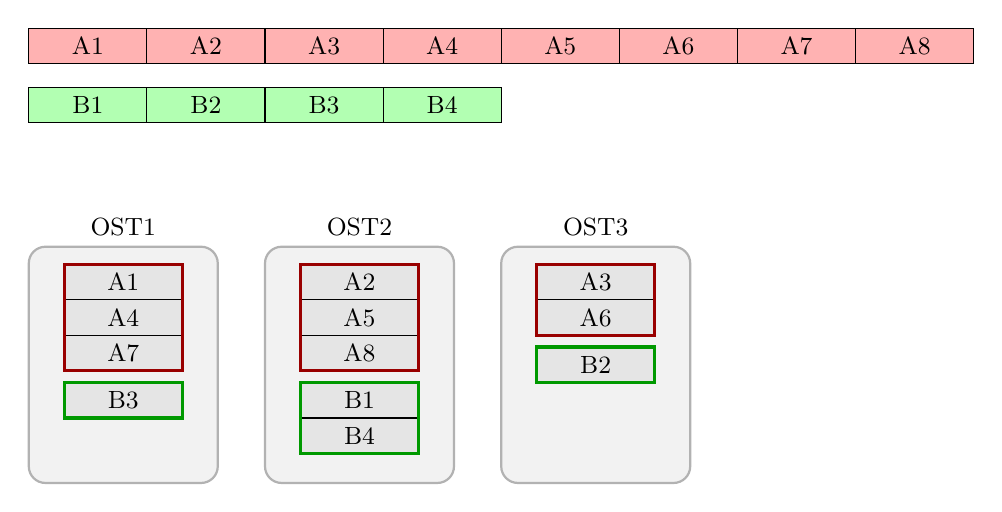
\begin{tikzpicture}[x=1.5cm,y=1.5cm,every node/.style={font=\small}]
            \node[block,a] (a1) at (0.5, -0.3) {A1};
            \node[block,a] (a2) at (1.5, -0.3) {A2};
            \node[block,a] (a3) at (2.5, -0.3) {A3};
            \node[block,a] (a4) at (3.5, -0.3) {A4};
            \node[block,a] (a5) at (4.5, -0.3) {A5};
            \node[block,a] (a6) at (5.5, -0.3) {A6};
            \node[block,a] (a7) at (6.5, -0.3) {A7};
            \node[block,a] (a8) at (7.5, -0.3) {A8};

            \node[block,b] (b1) at (0.5, -0.8) {B1};
            \node[block,b] (b2) at (1.5, -0.8) {B2};
            \node[block,b] (b3) at (2.5, -0.8) {B3};
            \node[block,b] (b4) at (3.5, -0.8) {B4};

            \node[ost,label=above:OST1] (ost1) at (0.8, -3) {};
            \node[ost,label=above:OST2] (ost2) at (2.8, -3) {};
            \node[ost,label=above:OST3] (ost3) at (4.8, -3) {};

            \node[block] (da1) at (0.8, -2.3) {A1};
            \node[block] (da2) at (2.8, -2.3) {A2};
            \node[block] (da3) at (4.8, -2.3) {A3};
            \node[block] (da4) at (0.8, -2.6) {A4};
            \node[block] (da5) at (2.8, -2.6) {A5};
            \node[block] (da6) at (4.8, -2.6) {A6};
            \node[block] (da7) at (0.8, -2.9) {A7};
            \node[block] (da8) at (2.8, -2.9) {A8};

            \node[block] (db1) at (2.8, -3.3) {B1};
            \node[block] (db2) at (4.8, -3.0) {B2};
            \node[block] (db3) at (0.8, -3.3) {B3};
            \node[block] (db4) at (2.8, -3.6) {B4};

            \node[object,minimum height=1.35cm,draw=red!60!black] (o1) at (0.8, -2.6) {};
            \node[object,minimum height=1.35cm,draw=red!60!black] (o2) at (2.8, -2.6) {};
            \node[object,minimum height=0.9cm,draw=red!60!black] (o3) at (4.8, -2.45) {};

            \node[object,minimum height=0.9cm,draw=green!60!black] (o4) at (2.8, -3.45) {};
            \node[object,minimum height=0.45cm,draw=green!60!black] (o4) at (0.8, -3.3) {};
            \node[object,minimum height=0.45cm,draw=green!60!black] (o4) at (4.8, -3.0) {};
        \end{tikzpicture}
    }

    \caption{Striping}
    \label{fig:striping}
\end{figure}

Figure~\ref{fig:striping} indicates how files are being split and distrubuted.
The red and green blocks on top represent file data, which is split into
eight and four blocks, respectively. The red file (file A) starts on OST1,
and the blocks are placed on OST 1 through 3 in order. The resulting red
block on OST1 consists of the data blocks a1, a4 and a7. This target block
is called the \textbf{object} of file A on OST1. Each object is internally saved
as a single file on the OST, using the filesystem present on that target.

The placement of file B (green) in this example starts on OST2, again creating
three objects on the OSTs. Only the first object contains more than one data
blocks, since the file is only four blocks in length.

Striping has multiple advantages for the Lustre architecture. Most importantly,
it describes a mechanism to distribute the data across the OSTs. Thus, the
client can write/read simultaneously to/from all OSSs involved, accumulating
the bandwith and disk speed limits for a higher total throughput. By striping
across multiple targets, the file size is also not limited to the size of
a single target anymore, allowing the user to store huge amounts of data
in a single file.

The block size and number of target objects is adjustable. In Lustre, these
attributes can be set as metadata on a per-tree or per-file level, giving
the administrator great control of the striping process and the ability to
fine-tune the setup for the user's needs.
